\documentclass[12pt,a4paper]{article}
\usepackage[utf8]{inputenc}
\usepackage[T1]{fontenc}
\usepackage[francais]{babel}
\usepackage{lmodern} %pack de police
\usepackage{eurosym}
\usepackage{graphicx}
\usepackage[left=2cm, right=2cm, top=2cm, bottom=2cm]{geometry}


\title{Contrôler sa maison à l'aide d'un Raspberry}
\author{\textsc{Essig} Meryll \and \textsc{Rocacher} Tamara}


\begin{document}
\maketitle
\vfill

\section*{Introduction}
  Pour réaliser le travail depuis notre présentation, nous avons dû étudier la communication entre le client et le serveur afin de pouvoir passer et traiter des configurations. En effet, cela permettra ensuite de paramétrer les scénarios sans recours à une recompilation.
\vfill
  \section*{Client}
  Ainsi, nous avons séparé le travail, avec d'une part le client, permettant à l'utilisateur de dialoguer avec le serveur domotique en lui envoyant des informations dans des fichiers de configuration, par le biais d'une interface graphique.\\
\vfill
  \begin{center}
  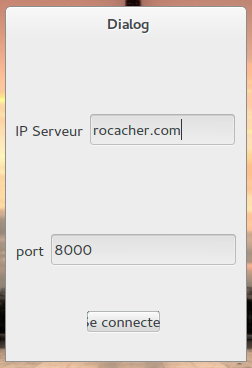
\includegraphics[scale=0.45]{connexion.png}
\end{center}
\vfill
\newpage
\begin{center}
  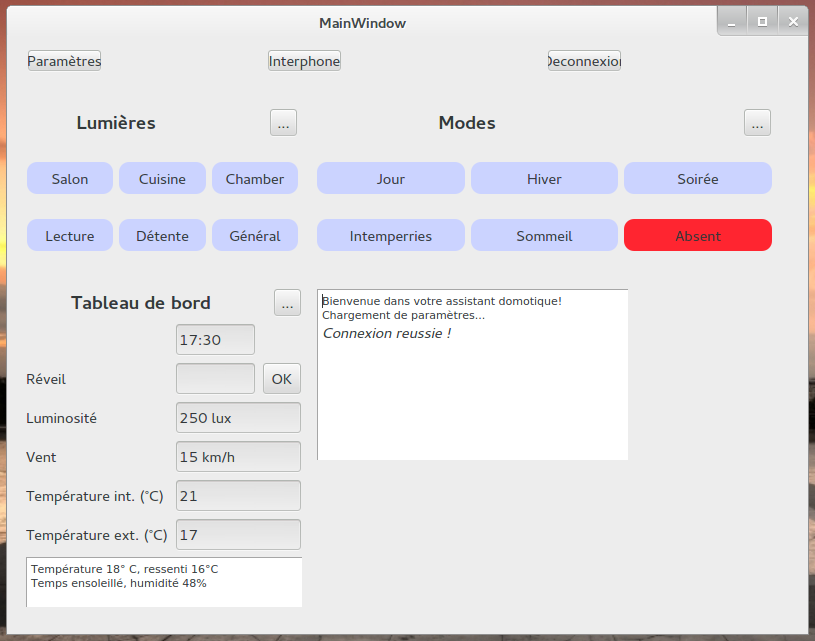
\includegraphics[scale=0.45]{mainWin.png}
\end{center}
  \\
  \newline
  L'utilisateur doit en effet pouvoir s'identifier, ajouter des composants ou les retirer pour ensuite en avoir le contrôle ou les soumettre à un ou plusieurs scénarios.
  D'autre part, l'utilisateur doit pouvoir se renseigner rapidement sur l'état des composants, qui pourra être affiché grâce a la réception d'informations envoyées par le serveur.

  \section*{Serveur}
  D'autre part, pour le serveur, nous avons fait le choix d'avoir un fichier de configuration qui restera statique pour un domicile donné :
  \begin{verbatim}
    port=8000
    language=fr-FR
    restartScenario=3600 ;Relire les scenarios pour modifications toutes les 3600 secondes
  \end{verbatim}
  Coté scenarios, nous concevons un format de fichier *.domo qui comportera une suite de règles et d'actions associées:
  \begin{verbatim}
    WHEN
    SUJET OPERATEUR VALEUR SUJET OPERATEUR VALEUR .....
    THEN
    COMPOSANT ETAT COMPOSANT ETAT ....
  \end{verbatim}

  Ainsi, cela pourra donner par exemple :
  \begin{verbatim}
    WHEN
    LUX > 300 TEMP > 20.2
    THEN
    1 1 3 0
  \end{verbatim}

  Cet exemple changera l'état du composant n°1 à ON et du n°3 à OFF lorsque la lumière est supérieure à 300 lux et la température supérieure à 20.2°C.

  Ce fichier pourra être modifié lorsque le client aura envoyé une nouvelle configuration, afin d'actualiser les conditions (paramétrage de scénarios) ou les composants (ajout, retrait,...).

\section*{Contraintes}
  L'implémentation du serveur et celle du client deviennent interdépendantes du fait du format de fichier personnalisé à traiter, et qui doit correspondre entre l'émission et la reception.
  Nous continuerons donc à faire un travail parallèle sur le client et le serveur, qui permettra de tester au fur et à mesure la création des fichiers, le transfert et le traitement.

\end{document}
